\chapter{Outer Tracker Luminometer}

The CMS Phase-2 Outer Tracker  (OT) system will provide a source of high rate physics objects: L1 track stubs.
In the OT DAQ architecture design, these objects are produced by the front-end electronics at full 40 MHz frequency~\cite{CERN-LHCC-2017-009}.
Studies of CMS Phase-2 simulations show excellent linearity in the counting of these objects up to the HL-LHC pileup.
These properties make this an excellent candidate for a precision luminometer with online functionality.
In the following sections the detector layout, a preliminary design of the data acquisition system, and the expected perfomace are described.


\section{Detector Layout and track stub reconstruction}


The design of the Phase-2 OT detector is described in The Phase-2 Upgrade of the
CMS Tracker Technical Design Report ~\cite{CERN-LHCC-2017-009} and shown here in Figure~\ref{fig:OT_layout}.
The layout consists of 6 barrel layers (3 TBPS + 3 TB2S) and 5 endcap (TEDD) disks.
The design of the  Phase-2 L1 trigger system requires the reconstruction of track stubs
in the front-end of the OT as a first step of the track reconstruction for the L1 trigger.
For the luminosity measurement, CMS detector simulations have been studied up to the HL-LHC expected pile-up,
these studies described below, show that the best precision can be obtained with the track stub counting from the barrel layer 6. 
The OT barrel layer 6 consists of 78 sensor ``ladders'' on each side of the CMS detector,
with each ladder containing 12 sensor modules as shown in Figure~\ref{fig:OT_ladder_stub}.
To ensure hermetic coverage, the sensors are staggered along the z direction within the ladder,
and the ladders are staggered along the phi direction as can be observed by the two radial positions in Figure~\ref{fig:OT_layout}.
The track stub reconstruction (right side of Figure~\ref{fig:OT_ladder_stub}) is performed with firmware algorithms
in the front-end electronics and the objects are transmitted to the back-end using high speed optical links.

\begin{figure}[h!]
\centering
\begin{subfigure}
\centering
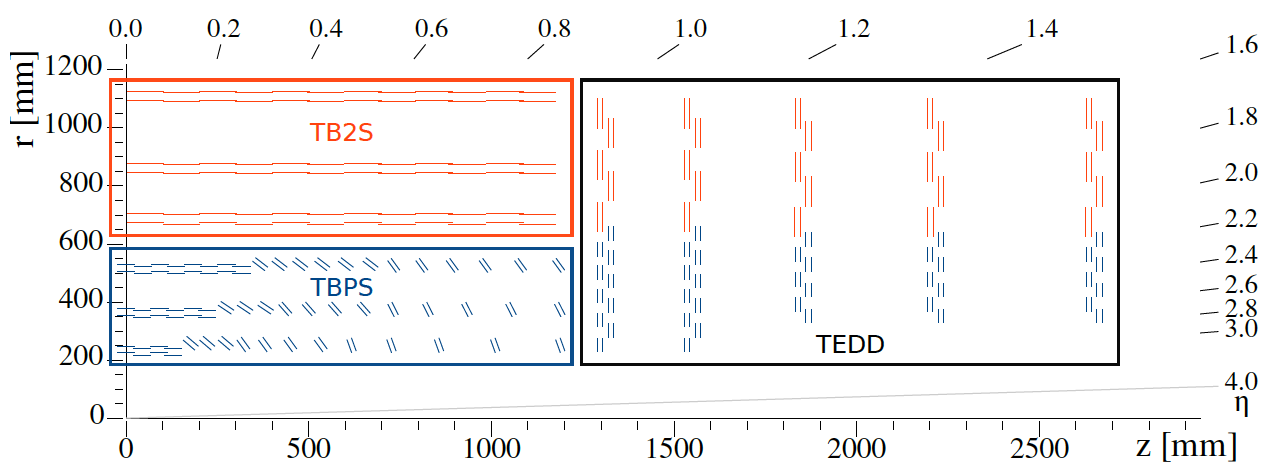
\includegraphics[width=.95\linewidth]{tex/Part2/fig/OT/OT-longitudinal.png}
\end{subfigure}
\caption{
  Longitudinal view of the CMS Phase-2 Outer Tracker layout  with two regions in the barrel (TB2S, TBPS) and the endcap region (TEDD).
  For the luminosity measurement the barrel outermost layer 6 in the TB2S part is used, this layer consists of 78 sensor ladders on each side of CMS.
}
\label{fig:OT_layout}
\end{figure}




\section{Data Acquisition}

A design of the OT DAQ including both the front-end and back-end systems is shown in Figure~\ref{fig:OT_DAQ}.
The back-end consists of Data, Trigger, and Control (DTC) boards which process the Trigger (TRIG) stream containting the track stub information. 
The list of track stubs reconstructed for each bunch crossing is transmitted in blocks of 8 bunch crossings to the DTC boards.
For the online luminosity measurement, the BRIL Histogramming firmware described in Chapter~\ref{sec:BRILDAQ}
will be installed in the DTC boards and run in synchronous mode
to count the number of track stubs in each bunch crossing  at regular integration intervals of approximately 1 second.
Each histogram module will be configured to integrate track stubs from one  sensor ladder.
The DTC boards process 3-6 ladders, and will be configured with the corresponding number of histogram module instances.
The readout of the luminosity histograms can be performed as part of the slow control of the OT back-end via IPBus network protocol
to the BRIL-DAQ system for further processing and storage.
The final calculation of the online luminosity is performed with software in the BRIL-DAQ and accounts for background subtractions (e.g. the afterglow physics noise)
and will filter unstable detector parts while applying the necessary weights to the normalization.
\textcolor{red}{(Here add a sentence about the availibility of this luminometer)}

Considering the rate of track stubs per ladder estimated with CMS simulations at pile-up of 200  (Figure~\ref{fig:OT_rates}),
the number of stubs per ladder expected is approximately 90,000 per bunch per second, requiring 17 bits of memory per bin of the luminosity histogram.
In addition, the stability of the modules must be tracked in time in order to maintain the necessary stability for the luminosity measurement.
This will be acomplished by propagating errors from the OT frontend and backend to the luminosity histograms
and filtering the modules in real time before computing the total ladder count, this will require additional memory for tracking these possible errors.
The total necessary memory per luminosity histogram is estimated using 32-bit memory words as follows:
3564 stub counting bins + 9 header + 2 static module mask + 192 online errors, for a total of 3767 words or 120 Kb per histogram.
In the case of DTC's with 6 ladders readout at 1 second intervals this corresponds to a data bandwidth of ~720 Kbps.
For the whole of the OT layer 6, a total of 156 lumi histograms, the total data rate received by the BRIL-DAQ will be approximately 18.8 Mbps.



\clearpage

\begin{figure}[h!]
\centering
\begin{subfigure}
  \centering
  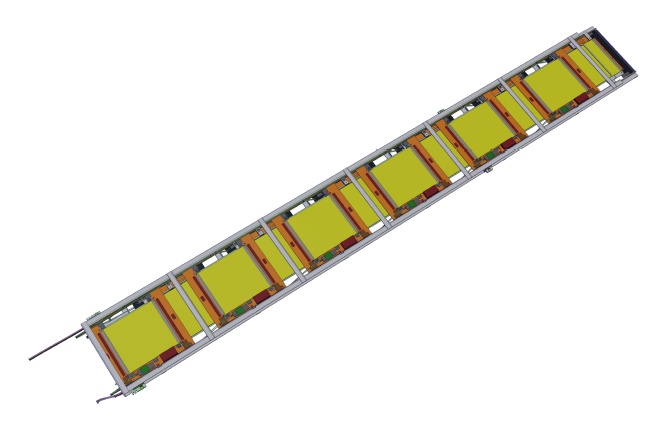
\includegraphics[width=.48\linewidth]{tex/Part2/fig/OT/OT-ladder.png}
\end{subfigure}
\begin{subfigure}
  \centering
  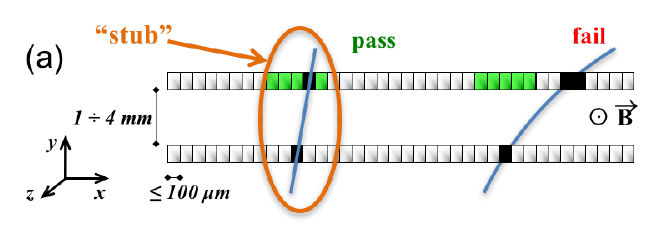
\includegraphics[width=.48\linewidth]{tex/Part2/fig/OT/OT-stub.png}
\end{subfigure}
\caption{
  Layout of one OT sensor ladder with 12 modules (left) and diagram of the track stub reconstruction (right) using the two sensor layers in each module.  
}
\label{fig:OT_ladder_stub}
\end{figure}



\begin{figure}[hbtp]
\centering
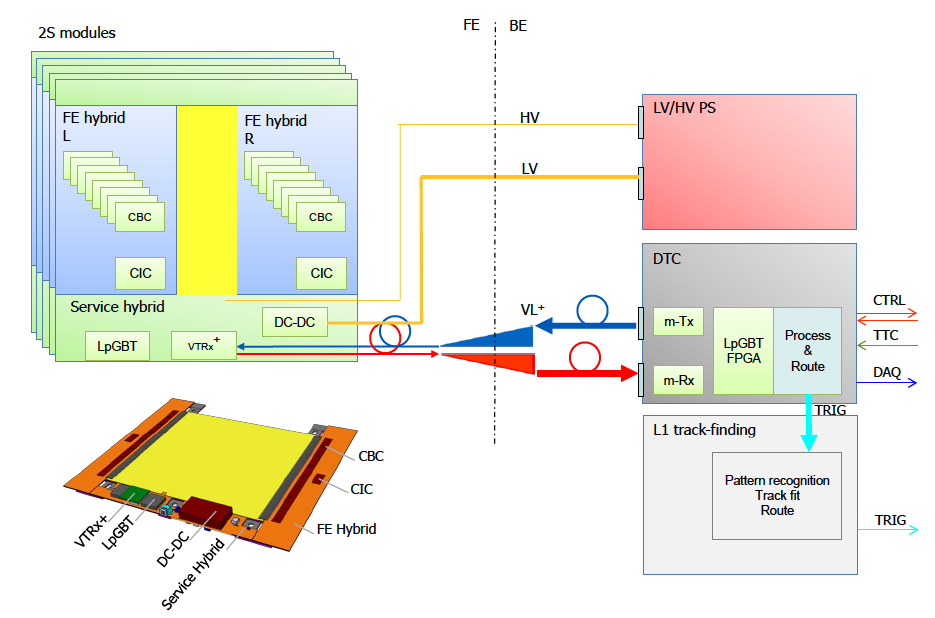
\includegraphics[width=.85\linewidth]{tex/Part2/fig/OT/OT-DAQoverview.png}
\caption{
  Design of the Phase-2 Outer Tracker front-end and back-end electronics~\cite{CERN-LHCC-2017-009}.
  The track stubs are reconstructed in the front-end, the back-end DTC boards will be configured with the BRIL luminosity histogramming firmware.  
}   
\label{fig:OT_DAQ}
\end{figure}


\clearpage

\section{Expected Performance}
%- Rates\\
%- linearity \\
%- statistical precision

The performance of the Phase II OT has been studied using detailed detector simulations for a wide range of pile-up scenarios. The samples have been privately produced using CMSSW version 11\_2\_0\_pre6 and a custom geometry that includes only the tracker volume with geometry versions 6.1.3 and 6.1.6 for the Inner and Outer Tracker, respectively.They also contain simulated effects from front-end electronics, specifically for the OT 2S modules the CBC hit detection mode is set to latched. Similar to what was done for TEPX simulations (see section \ref{sec:TEPX_sim}), the process that has been used to generate these samples is a single-neutrino event overlaid with a variable number of minimum-bias events to simulate pile-up. 

To test the linearity, the number of stubs is histogrammed per event for each layer of the OT. The mean of these distributions is then plotted as a function of pile-up, and a line is fitted to the lowest pile-up points (between 0 and 2) and then extrapolated to higher values, up to a pile-up of 200. Figure \ref{fig:OT_linearity} shows the linearity of stubs for all OT barrel layers. The deviation from a perfectly linear behaviour is presented in figure \ref{fig:OT_deviation}, where it can be seen that layer 6 has a deviation of less than 1\% across the full pile-up range.

\begin{figure}[h!]
\centering
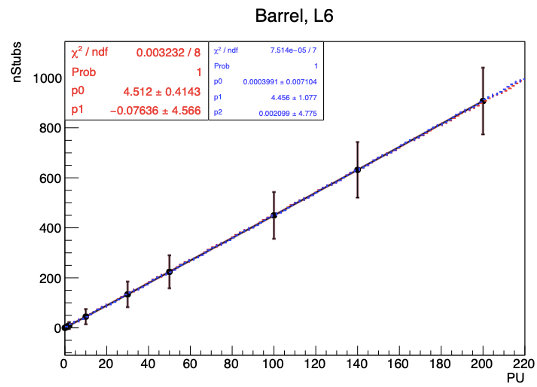
\includegraphics[width=.6\linewidth]{tex/Part2/fig/OT/OT-linearity.png}
\caption{
 Average number of track stubs per event as a function of pile-up determined from the CMS Phase II simulation showing a linear behaviour. \nts{PLACEHOLDER: To be replaced with a linearity plot including all barrel layers.}
} 
\label{fig:OT_linearity}
\end{figure}

\begin{figure}[h!]
\centering
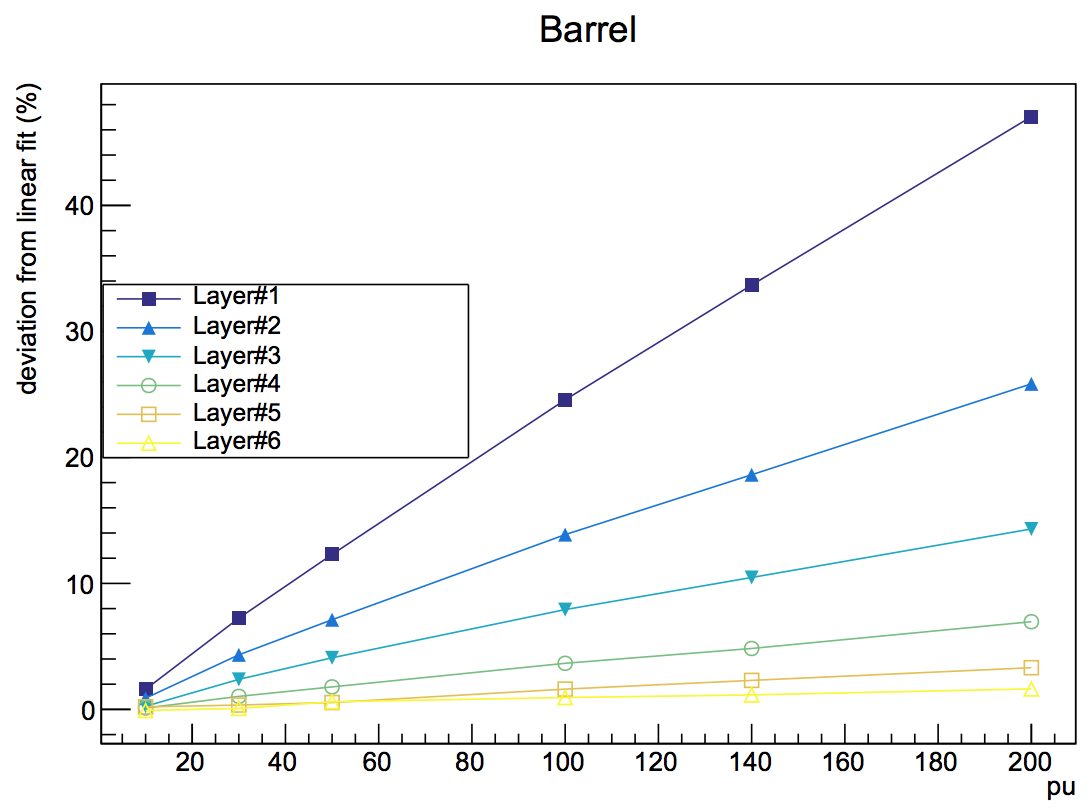
\includegraphics[width=.6\linewidth]{tex/Part2/fig/OT/OT-deviation.png}
\caption{
 Deviation from linearity for all barrel layers of the OT. \nts{PLACEHOLDER: To be replaced with plot using CMS style.}
}
\label{fig:OT_deviation}
\end{figure}

Another important figure of merit for the performance of the OT as a luminometer is the statistical precision that can be achieved. Figure \ref{fig:OT_rates} shows the average number of stubs per event per ladder in layer 6, obtained from the simulations described above. The maximum total rate for the pile-up step of 200 is found to be of 902 stubs per event for Physics and of 2.255 for vdM conditions. With these counts, and considering a trigger readout rate of 40~MHz and an integration period of 1~s (30~s), a statistical precision of 0.03\% (0.115\%) per bunch-crossing is expected for Physics (vdM) conditions.   

\begin{figure}[h!]
\centering
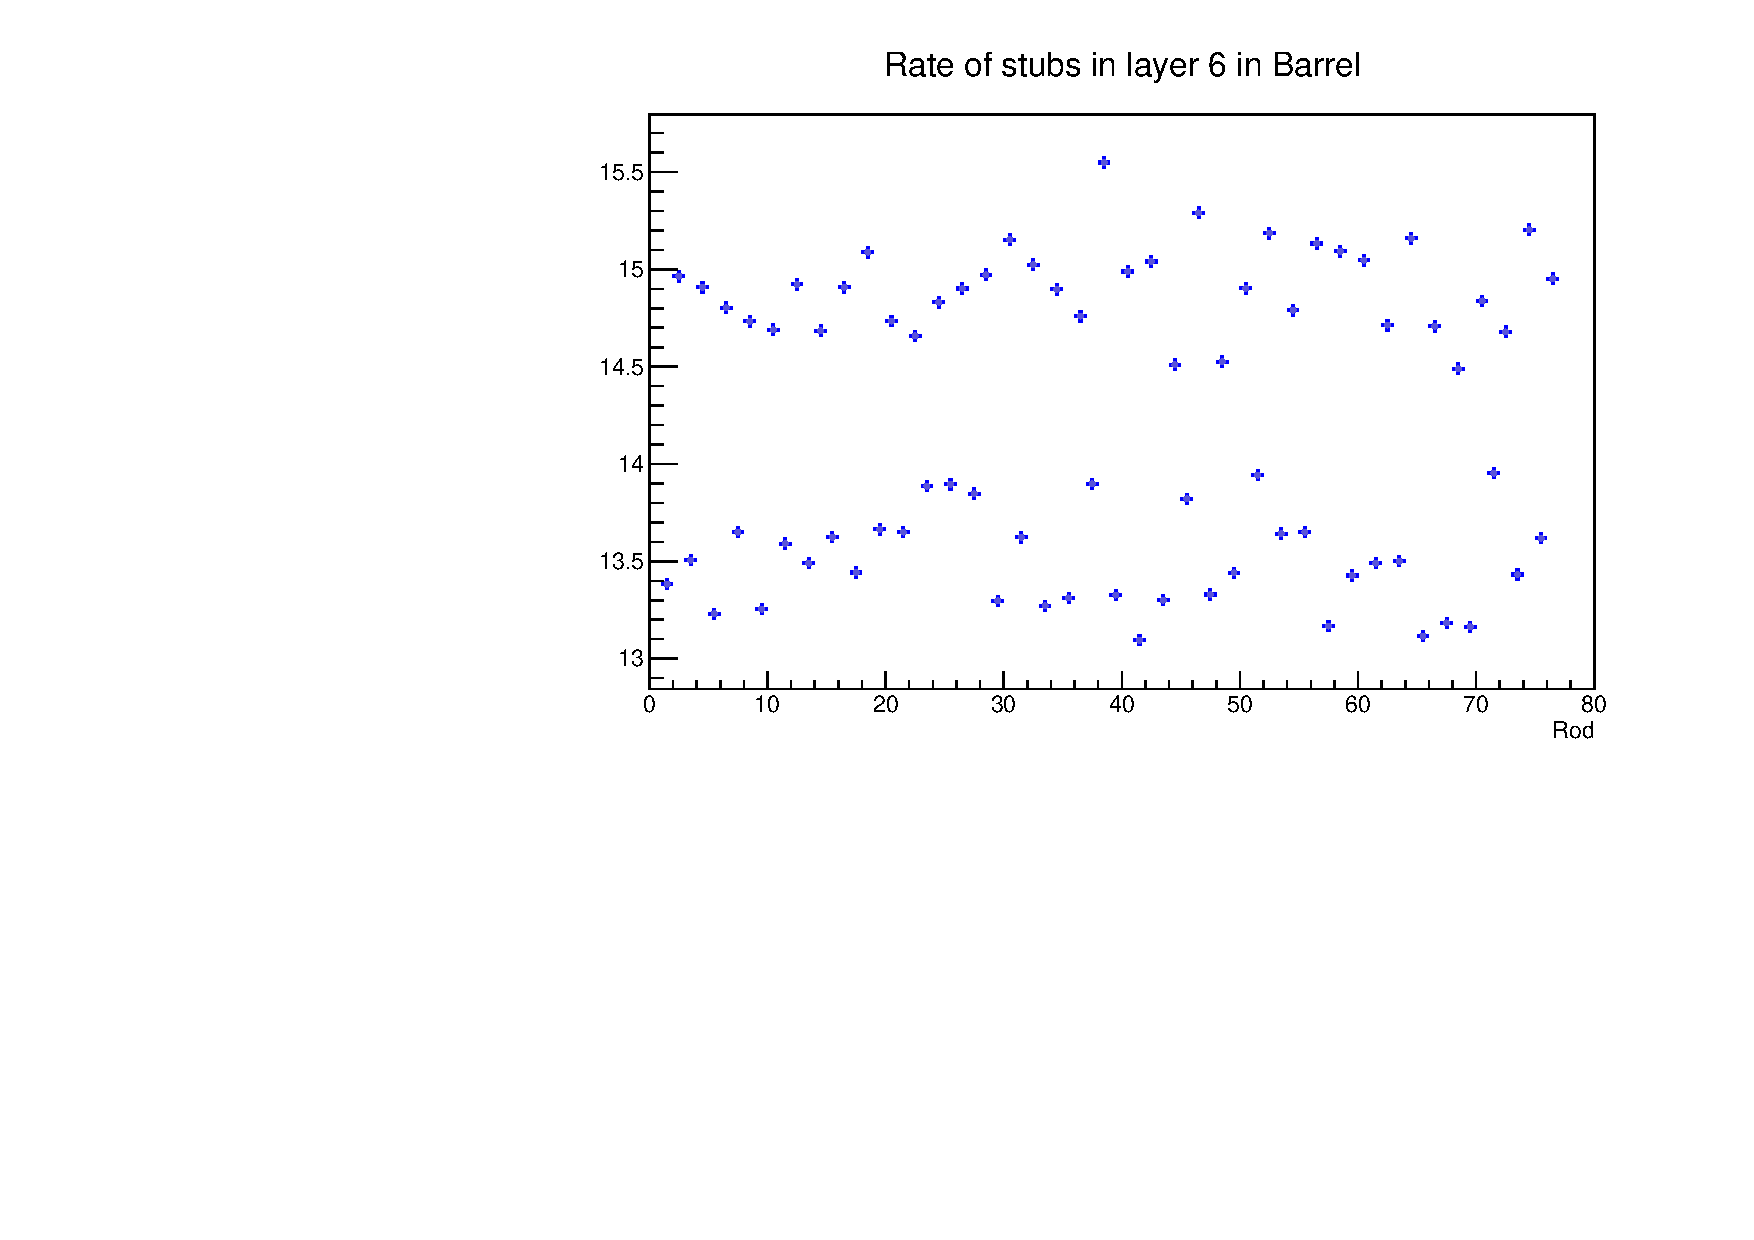
\includegraphics[width=.6\linewidth]{tex/Part2/fig/OT/OT-Rates.pdf}
\caption{
  Average number of track stubs per event per ladder as a function of the ladder id.
  The rate is determined from the CMS Phase II simulation for a pile-up of 200. \nts{PLACEHOLDER: To be replaced with plot using CMS style.}
}
\label{fig:OT_rates}
\end{figure}




